\documentclass{article}
\usepackage[utf8]{inputenc}
\usepackage{amsthm,amsmath,amssymb}
\usepackage[margin = 1in]{geometry}
\usepackage{biblatex,tikz}
\usepackage{pgfplots}
\addbibresource{ref.bib}



\makeatletter
\g@addto@macro\@floatboxreset\centering
\makeatother

\usepackage[ numbered,autolinebreaks,useliterate]{mcode}


\newcommand{\bx}{{\bf x}}
\newcommand{\bb}{{\bf b}}
\newcommand{\bh}{{\bf h}}
\newcommand{\br}{{\bf r}}
\newcommand{\bk}{{\bf k}}
\newcommand{\bu}{{\bf u}}
\newcommand{\bv}{{\bf v}}
\newcommand{\bp}{{\bf p}}
\newcommand{\by}{{\bf y}}

\newcommand{\R}{\mathbb{R}}
\newcommand{\C}{\mathbb{C}}
\newcommand{\V}{\mathbb{V}}
\newcommand{\beq}{\begin{equation}}
\newcommand{\eeq}{\end{equation}}

\DeclareMathOperator*{\argmin}{arg\,min}

\newtheorem{thm}{Theorem}[section]
\newtheorem{lemma}{Lemma}[section]
\newtheorem{defn}{Definition}[section]
\newtheorem{prop}{Proposition}[section]


\theoremstyle{remark}
\newtheorem*{remark}{Remark}




\title{Finding $A^{-1}{\bf b}$ with The Conjugate Gradient Method}
\author{Lee Fisher}


\begin{document}

\maketitle
\abstract{This document is a short explanation of how the conjugate gradient method can be used to quickly evaluate the inverse of symmetric positive definite matrix. We start by reframing the Poisson equation on an interval in terms of evaluating the inverse of an SPD matrix. We start with attempting to find a solution with a simple gradient descent and then we use more sophisticated linear algebra to make gradual improvements to the algorithm. We will include Matlab code snippets throughout the derivation to emphasize how the algorithm can be implemented, we also discuss limitations, and the convergence rate of this method. We conlcude with a brief discussion of preconditioning. You will find a full working example in this github folder.}

\section{Introduction}

This is a method for solving a linear system of equations originally discovered by Hestenes and Stiefel in \cite{hest52}, this presentation of the method draws from \cite{KelleyCT}, \cite{GreenbaumA}, and lecture notes from a graduate course on Numerical Analysis at UC Irvine \cite{lchen}.

There are many variations of the Conjugate Gradient method and also ways to apply it to matrices that are not symmetic prositive definite. This is a commonly used method to quickly solve a sparse linear system it is conceptually similar to the well known method of gradient descent; but by focusing the alternate geometry that the inner product associated to an SPD-matrix bestows on $\mathbb{R}^n$, we can in some cases drastically improve on the efficiency of the method of gradient descent. 



\section{Poisson's Equation on an Interval}

Consider the following well known differential equation,
\begin{align}
\label{eq:p1d}
-u''(x) &= f(x) \text{ for } x\in (0,1)\\ \nonumber
u(0) &= g_0\\ \nonumber
u(1) &= g_1.
\end{align}

This may seem too simple, after all an analytic solution is easily available. 

\beq
u(x) = -\int_0^x \int_0^t f(s)dsdt + C_{1,g} + C_{2,g}x.
\eeq

This is nice and convenient, and the methods of numerical integration are fast and efficient. However this strategy will not work, or at least not nearly as easily in higher dimensions.
\begin{align}
\label{eq:pnd}
-\Delta u &= f(x) \text{ for } x\in \Omega \subset \mathbb{R}^n\\ \nonumber
u|_{\partial \Omega} &= g(x)
\end{align}

Our strategy is not to solve by integrating but by matrix-ifying our equation. This, discretization strategy is quite powerful and it will work in any dimension; but focusing on the  version is will provide enough generality to communicate all the important ideas. 

We will replace $\eqref{eq:p1d}$ with an approximate problem. Consider a partition of the unit interval into equal pieces, each of width $h= 1/N$. When $u(x)$ is restricted to the endpoints  of the partition, it can be thought of as a vector with $n+1$ entries. So $\bu_k = u(kh)$ for $k = 0, \dots, N$. There is a nice way to estimate the derivative using only the points in our partition.  
\beq
\label{eq:applap}
\lim_{\Delta x \to 0} \frac{u(kh+\Delta x) -2u(kh) + u(kh-\Delta x)}{\Delta x^2}\approx \frac{\bu_{k+1} - 2\bu_k + \bu_{k-1}}{h^2} = u''(kh) + O(h^2)
\eeq

This error estimate can be verified by expanding $u(x)$ in Taylor series. From the last equality in $\eqref{eq:applap}$ and a little algebra, we can rephrase $\eqref{eq:applap}$ as an $(N-1)\times(N-1)$ linear system. 

\beq
\label{eq:A}
\begin{bmatrix}
2 & -1 & 0 & \dots & 0   \\
-1  & 2 & -1 & \dots & 0  \\
0  & -1 & 2 & \dots & 0 \\
\vdots & \vdots & \vdots & \ddots & \vdots \\
0 & 0 & 0 & \dots & 2
\end{bmatrix}
 \begin{bmatrix}
u_1\\ 
u_2\\
u_3\\
\vdots\\
u_{N-1}
\end{bmatrix}
= 
\begin{bmatrix}
h^2f_1 - g_0\\
h^2f_2 \\
h^2f_3 \\
\vdots\\
h^2f_{N-1} - g_1
\end{bmatrix}
\eeq

It is not hard to verify that the tridiagonal matrix on the left hand side really is  symmetric and positive definite. It is straightforward to construct our matrix in MATLAB. 

\begin{lstlisting}
e = ones(N-1,1);
A = spdiags([-1*e 2*e -1*e], -1:1, N-1, N-1);
\end{lstlisting}

We will also intialize our problem by choosing $f(x) = \sinh(x)$, $g_0,g_1 = 0$, and $N = 100$. This gives us a consistent benchmark to judge the speed of the different algorithms.
\begin{lstlisting}
N= 100;
h = 1/N;
pts = h:h:1-h;
f = h*h*sinh(pts);
g = [0,0];
f(1) = f(1) - g(1);
f(N-1) = f(N-1) - g(2);
\end{lstlisting}

The first algorithms we introduce are too slow and the later algorithms are too fast, so we will adjust the size of $N$ as we go along. 


\section{The $A$-linear algebra.}

We will focus on the abstract problem for the time being. We want to evalue to inverse of an $SPD$ matrix $A$ at a particular point. 

\begin{align}
\label{eq:main}
A\bx = \bb &\implies \bx_* = A^{-1}\bb. &\text{ We want to evaluate the inverse.}\\
A &= A^t. &\text{ $A$ is symmetric.}\\
\text{ For all $\bx \neq 0$, }\langle \bx, A\bx \rangle &= \bx^t A \bx > 0. &\text{ $A$ is postive definite.}
\end{align}

The goal is calculate $\bx_*$, and if there is a trade off between finding an exact solution and finding an approximate solution quickly we will prefer the quick solution. The approach that is most well known is Gaussian elimination, and this will give the exact solution, but this process can be extremely, even infeasibly slow when unleased on a sufficiently large system. We introduce some terminology to clarify what we mean by approximate. 

\begin{defn}[Error] If $\bx$ is a approximation to $\bx_*$ then we will define respectively the error vector and the error of the approximation as 
\begin{align}
{\bf \epsilon}_\bx &= \bx_*-\bx\\
\|\epsilon_\bx\| &= \|\bx_* - \bx \|
\end{align}
\end{defn}

\begin{defn}[Residual] We say that a vector $\bx$ is an approximation to $\bx_*$ then we say the residual of the approximation is, 
\beq
\br_\bx = \bb - A\bx .
\eeq
\end{defn}

We will omit the subscripts when the meaning is clear from context. Intuitively the error simply tells us how far our approximation misses the mark. Unfortunately we can't get our hands on the error exactly because that would require knowing $\bx_*$. The residual will work as an auxillary, more tangible, measurement of the error. We can use the fact that $\bb = A\bx_*$ to see this more clearly. 

\beq
\br = \bb - A\bx = A\bx_* - A\bx = A(\bx_* - \bx) = A\epsilon.
\eeq
This is a reasonable substutite, it is straightforward to compare the size of the error to the size of the residual. 
\beq
\|\br \| = \sqrt{\langle A\epsilon , A\epsilon \rangle} = \|\epsilon\|\sqrt{ \left\langle A\frac{\epsilon_x}{\|\epsilon\|} , A\frac{\epsilon}{\|\epsilon\|} \right\rangle} \leq \|\epsilon\| \sqrt{ \sup_{\|\bu\|=1}\langle A\bu, A\bu \rangle} = \|\epsilon\| \cdot \|A\|
\eeq

This is what we will work with to measure error but this has some limitations. We assume that calculating $\|A\|$ is an expensive task, so without knowledge of the norm it could be difficult to judge whether the resolvent actually corresponds to a good approximation. If $\|A\| $ is large then it is possible that a large resolvent could actually correspond to a good approximation and if the norm is small we would have the opposite problem. This first issue is solved by making sure to judge the quality of $\|r\|$ by how it compares to the size of $\|b\|$. 

There is another issue however. Since we assumed that $A$ is SPD this implies that it has only positive real eigenvalues, an equivalent statement is to say that the image of a sphere in $\R^n$ under $A$ will be an ellipsoid. If this ellipsoid is highly eccentric, so the largest axis is much longer than the shortest axis, (i.e. the largest eigenvalue is much larger than the smallest eigenvalue) then the resolvent can only work as a crude estimate of the error. We call these problem causing matrices \textit{ill-conditioned} and we will cover how to deal with them in more detail in section 5, see \cite{hest52} \textsection 18 for an explicit pathological example. 

Our strategy is to use an iterative process to create a sequence of approximations, $\bx_0, \bx_1,\dots$ and a corresponding sequence of resolvents $\br_0, \br_1,\dots$ we will halt the process once the norm of the resolvent becomes small, and when $A$ is well-conditioned this approach is going to work. For simplicity we will use the convention that $\bx_0= 0$ and $\br_0 = \bb$.

\begin{defn}[Geometry of $A$.] We define the $A$-inner product and the $A$-norm respectively
\begin{align}
\langle \bu, \bv \rangle_A &= \langle \bu, A \bv \rangle = \langle A\bu,  \bv \rangle\\
\|\bu \|_A &= \sqrt{\langle \bu, A\bu \rangle}
\end{align}
\end{defn}

Since $A$ is SPD, $\langle \cdot, \cdot \rangle_A$ really is an inner product and $\| \cdot \|_A$ really is a norm. The analogy continues though, here is more terminology to discuss the geometry associated to $A$. 

\begin{defn}[Conjugate Vectors]  $\bu$ and $\bv$ are conjugate if they are $A$-orthogonal, that is $\langle \bu , \bv \rangle_A = 0$.
\end{defn}

\begin{defn}[$A$-Projection.] If $S$ is a subspace of $\R^n$ we can define the $A$-projection of $\bu$ onto $S$ as the unique vector in $S$ which satisfies the following:
\beq
\langle \text{\normalfont Proj}_S^A \bu, \bv \rangle_A = \langle \bu,\bv \rangle_A \text{ for all }\bv \in S.
\eeq
\end{defn}

This definition is nice, but it does not tell us exactly \textit{how} to calculate the $A$ projection. Thankfully this is completely analogous computing orthogonal projections in $\mathbb{R}^n$ in general. Suppose $S = \text{span}\{\bv_1, \dots \bv_k\}$, and $\{\bv_i\}$ are mutually conjugate then

\beq
\label{eq:Proj}
\text{Proj}^A_S \bu = \sum_{i=1}^k \frac{\langle \bu , \bv_i \rangle_A}{\langle \bv_i , \bv_i \rangle_A}\bv_i
\eeq

These concepts are crucial to the method. Suppose that we had a collection of $n$ mutually conjugate vectors $\bp_1, \bp_2, \dots \bp_n$. Then we could make short work of our problem. There would be some real numbers $\{\alpha_i\}_{i = 1,\dots n}$ such that, 
\beq
\label{eq:alphai}
\bx_* = \sum_{i=1}^n \alpha_i \bp_i
\eeq

But since the $\bp_i$ are mutually conjugate, calculating the $\alpha_i$ is simple. We can take the $A$-inner product of $\bx_*$ with $\bp_j$,
\beq
\label{eq:alphai2}
\langle \bp_j, \bx_* \rangle_A = \sum_{i = 1}^n \alpha_i \langle \bp_j, \bp_i\rangle_A = \alpha_j \langle \bp_j , \bp_j \rangle_A.
\eeq
But on the other hand we have that,
\beq
\label{eq:alphai3}
\langle \bp_j, \bx_* \rangle_A = \langle \bp_j, A\bx_*\rangle = \langle \bp_j, \bb \rangle.
\eeq
We simply solve for the $\alpha_j$ and find our solution. 
\beq 
\bx_* = \sum_{i=1}^n \frac{\langle \bp_i, \bb \rangle}{\langle \bp_i, \bp_i\rangle_A} \bp_i. 
\eeq

Of course this is unrealistic, but it is a good conceptual starting point. Computing and storing the entire conjugate basis for $\R^n$ is going to be slow and also require a lot of space. We will be able to reformulate the idea in terms of an iterative process. This will work similarly to gradient descent, but instead of strictly following the flow of the gradient we will impose the condition that the residual of the next step is $A$-orthogonal to the subspace spanned by the previous residuals.

\section{The Conjugate Gradient Method}


\begin{figure}[h]
\begin{tabular}{cc}
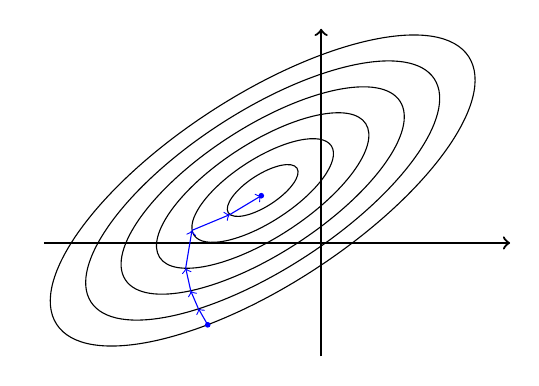
\begin{tikzpicture}[scale = 0.8]
\draw[->,thick] (-5.4,0.3)--(2,0.3);
\draw[->,thick] (-1,-1.5)--(-1,3.7);
    \foreach \i in {1,2,3,4,5,6}{
        \draw[rotate=33] (-1,2) ellipse (1.3*\i/2 and 0.5*\i/2);
        }
\coordinate (A) at (-2.8,-1);
    \filldraw [blue] (A) circle (1pt);
\coordinate (B) at (-2.8-0.15,-1+0.26);
\coordinate (C) at  (-2.8-0.15-0.12,-1+0.26+0.28);
\coordinate (D) at (-2.8-0.15-0.12-0.08,-1+0.26+0.28+0.36);
\coordinate (E) at (-2.8-0.15-0.12-0.08+0.1,-1+0.26+0.28+0.36+0.6);
\coordinate (F) at (-2.8-0.15-0.12-0.08+0.1+0.6,-1+0.26+0.28+0.36+0.6+0.25);
\coordinate (G) at (-2.8-0.15-0.12-0.08+0.1+0.6+0.5,-1+0.26+0.28+0.36+0.6+0.25+0.3);
    \filldraw [blue] (G) circle (1pt);
\draw[blue,->] (A)->(B);
\draw[blue,->] (B)->(C);
\draw[blue,->] (C)->(D);
\draw[blue,->] (D)->(E);
\draw[blue,->] (E)->(F);
\draw[blue,->] (F)->(G);
\end{tikzpicture} & 
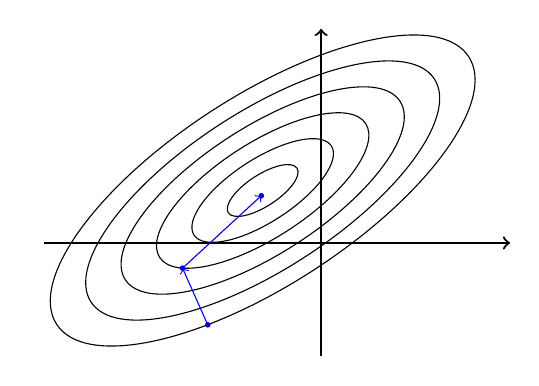
\begin{tikzpicture}[scale = 0.8]
\draw[->,thick] (-5.4,0.3)--(2,0.3);
\draw[->,thick] (-1,-1.5)--(-1,3.7);
    \foreach \i in {1,2,3,4,5,6}{
        \draw[rotate=33] (-1,2) ellipse (1.3*\i/2 and 0.5*\i/2);
        }
\coordinate (A) at (-2.8,-1);
    \filldraw [blue] (A) circle (1pt);
\coordinate (B) at (-2.8-0.4,-1+0.9);
    \filldraw [blue] (B) circle (1pt);
\coordinate (G) at (-2.8-0.15-0.12-0.08+0.1+0.6+0.5,-1+0.26+0.28+0.36+0.6+0.25+0.3);
    \filldraw [blue] (G) circle (1pt);
\draw[blue,->] (A)->(B);
\draw[blue,->] (B)->(G);
\end{tikzpicture}
\end{tabular}
\caption{Gradient descent vs. conjugate gradient method.}
\end{figure}


Notice we can rephrase problem \eqref{eq:main} in terms of minimizing a convex function.

\beq
\varphi(\bv) = \tfrac{1}{2}\|\bv\|_A^2 - \langle \bb, \bv \rangle 
\eeq
\beq
A\bx = \bb \iff \bx = \argmin_{\bv \in \R^n} f(\bv)
\eeq


For this simple convex function we have a nice expression for the gradient. 
\begin{equation}
-\nabla \varphi(\bx) = \bb - A\bx  = \br_{\bx}.
\end{equation}

The negative gradient at $\bx$ is simply the corresponding residual. Applying gradient descent is going to be our first attempt at solving the problem. We will use $\alpha$ for the step size. 

\subsection{Algorithm 1: Gradient Descent}
\begin{lstlisting}
function x = Gradient_Descent(A, b, tol, alpha, MaxIter)
x = zeros(length(b),1);
r = b;
k = 0;   
tol = tol*norm(f);
    while norm(r) >= tol && k < MaxIter
        r = b- A*x;
        x = x + alpha*r;
        k = k+1;
    end
end
\end{lstlisting}

This is easy to understand but it is not very good. To get an idea of how not efficient this code is, when $N = 100$ and $\alpha = 10^{-5}$, it takes a full 60 seconds for the code to compute an answer that has a relative error of $0.005\%$. Simply running $A\setminus f$ to compute the answer takes $0.07$ milliseconds for comparison. Toying with $\alpha$ and other parameters can speed up the code or make it more accurate. If we were stuck with just \textit{some} convex function it can be hard to do better than this, but we know more about our problem than just convexity. 


We can make an improvement by having $\alpha_k$ instead of just $\alpha$. What if choose the $\alpha_k$, so that the update from $\bx_{k+1}$ to $\bx_k$ makes $\varphi(\bx_{k+1})$ as small as possible. This is the steepest gradient descent algorithm. In equations we want that
\beq
\alpha_k = \argmin_{\alpha \in \R} \varphi(\bx_k + \alpha\br_k ).
\eeq
It is actually not that hard to find the minimum of this function. 
\beq
\alpha_k \br_k = \text{Proj}^A_{\br_k}(\bx_* - \bx_k) = \frac{\langle \br_k, \bx_*-\bx_k \rangle_A }{\langle \br_k , \br_k \rangle_A} \br_k = \frac{\langle \br_k, \br_k \rangle }{\langle \br_k , \br_k \rangle_A} \br_k.
\eeq
By using the $A$-projection we can choose $\alpha_k$ so that $\bx_k + \alpha_k\br_k$ is the closest point (measured in the $A$-norm) to $\bx_*$ on the line spanned by $\{\bx_k + \alpha \br_k \}$ as $\alpha$ ranges over $\R$. This will also minimize the value of $\varphi$ along the line $x_k + \alpha \br_k$. From this we get an improved gradient descent algorithm. 


\subsection{Algorithm 2: Steepest Gradient Descent}
\begin{lstlisting}
function x = Steepest_Gradient_Descent(A, b, tol, MaxIter)
x = zeros(length(b),1);
r = b;
k = 0;   
tol = tol*norm(b);
    while norm(r) >= tol && k < MaxIter
        r = b- A*x;
        alpha = (r'*r)/(r'*(A*r));
        x = x + alpha*r;
        k = k+1;
    end
end
\end{lstlisting}

This is a vast improvement from regular gradient descent; this program does the same job $(N=100)$ in only 23ms. Not bad, but $A\setminus \bb$ solves the problem in 0.05ms so we can go a lot faster. When we try $N = 1,000$ steepest gradient descent starts to sputter though, it takes 7s to find the inverse, but $A\setminus \bb$ still only takes 0.06ms. Our algorithm is not guaranteed to terminate after a fixed point, if $A$ is even somewhat ill-conditioned, then the steepest gradient method could still zig-zag through the level curves for a quite a while before coming close to a solution. As we will see later, $A$ is in fact ill conditioned for large values of $N$. 

We introduce the first CG method as a modification of the steepest gradient descent algorithm. The crux of the idea is to use an $A$-orthogonal set of vectors $\bp_k$, instead of the residuals, to update our guesses. At each step of the process we will use $\br_k$ to construct a new vector $\bp_k$ which is conjugate to $S_{k-1} := \text{span}\{\bp_0, \dots \bp_{k-1} \}$ and then use $\bp_k$ as the direction to move from $\bx_k$ to $\bx_{k+1}$. 

\subsection{Algorithm 3.0: CG Method (sketch)}
\begin{enumerate}
\item Initialize with $\bx_0=0$ and $\br_0 = \bp_0 = \bb$.
\item Repeat the following steps until $\|\br_k\|$ is small.
\item Select a step size $\alpha_k$.
\item Update our guess $\bx_{k+1}  = \bx_k + \alpha_k \bp_k$.
\item Compute the residual $\br_{k+1} = \bb - A\bx_{k+1}$,
\item and the new conjugate direction $\bp_{k+1} = \br_{k+1} - \text{Proj}^{A}_{S_k}\br_{k+1}$.

\end{enumerate}


We will simplify our notation going forward a little bit by saying $\Pi^k  = \text{Proj}^A_{S^k}$. For this algorithm there is only a description and no accompanying code for this sketch because of two glaring issues, picking the best $\alpha_k$ and computing $\Pi^k\br_{k+1}$. For the $\alpha_k$,  when we are using the $\bp_k$ as our directions instead of the residuals we have a better option than simply being greedy with the objective function. Recall \eqref{eq:alphai}, since we forced the $\bp_k$ to be mutually conjugate we can take advantage of this and select the $\alpha_i$ so that our algorithm must terminate in $n$ steps. From equations \eqref{eq:alphai2} and \eqref{eq:alphai3} we see that 
\beq
\alpha_k = \frac{\langle \bb , \bp_k \rangle}{\langle \bp_k , \bp_k \rangle_A}
\eeq

The other problem is calculating $\Pi^{k-1}\br_k$. From \eqref{eq:Proj} we have one way to compute the projection. 

\beq
\label{eq:pik1}
\Pi^{k-1}\br_k = \frac{\langle \br_k , \bp_{k-1}\rangle_A}{\langle \bp_{k-1}, \bp_{k-1}\rangle_A}\bp_{k-1} + \Pi^{k-2}\br_k = \sum_{j=1}^{k-1}\frac{\langle \br_k , \bp_j\rangle_A}{\langle \bp_j, \bp_j\rangle_A}\bp_j.
\eeq

If we try to put this into our code it will be wildly inefficient and waste not only time but also space. More insight into the linear algebra of our setup reveals that we actually do not need to compute all of those dot products in order to find the projection. 

\begin{lemma}
\label{lem:magic}
The vector $\br_k$ is $A$-orthogonal to $S_{k-2}$, that is $\Pi^{k-2}\br_k = 0$ (the cases where $k = 0,1$ are exceptional, but also trivial).
\end{lemma}

\begin{proof} This proof is a little unintuitive. First we show that $\br_k \perp S_{k-1}$, then from there we can prove that $\br_k$ is $A$-orthogonal to $S_{k-2}$.  At each step our algorithm chooses the $\alpha_{k-1}$ so that $\bx_k$ is the closest point (in the $A$-norm) to $\bx_*$ in the space $S^{k-1}$. In equations this means that,
\beq 
\bx_k = \Pi^{k-1} \bx_*.
\eeq

We can rewrite this to get the following,
\begin{align}
\bx_* - \bx_k &= (I-\Pi^{k-1})\bx_* \implies (\bx_* - \bx_k) \perp_A S_{k-1} \\
&\implies A(\bx_* - \bx_k) \perp S_{k-1} 
\implies \br_k \perp S_{k-1}. 
\end{align}

Remember that $(I - \Pi_S)$ is a projection onto $S^\perp$. Since $\br_0 = \bp_0 = \bb$ and $\br_k\perp S_{k-1}$ it means that, by induction, $\br_{k} \in S^k$ for all $k$. This is neat, in particular we have that the $\br_k$ and $\bp_k$ will span the same subspaces. There is a recursive way to write the resolvent
\begin{align}
\br_{k} &= \bb - A\bx_k = \bb-A\bx_{k-1} + A\bx_{k-1} - A\bx_k \\
\br_{k} &=  \br_{k-1} - \alpha_{k-1}A\bp_{k-1}. 
\end{align}

Suppose that $0 \leq i \leq k-2$, from the previous equation we see that
\beq 
A\bp_{i} \in \text{span}\{\br_{i}, \br_{i+1}\} \subset S_{i+1} \subset S_{k-1}.
\eeq

From the fact that $\br_k \perp S_{k-1}$, we can reach our conclusion, for all $i$ with $ 0 \leq i \in k-2$ we have,  
\beq
\br_k \perp S_{k-1} \implies \br_k \perp A\bp_{i} \implies \br_k \perp_A \bp_{i} \implies \br_k \perp_A S_{k-2}.
\eeq
\end{proof}

From this lemma we can find a more efficient expression for $\bp_{k+1}$.  
\beq 
\bp_{k+1} = \br_{k+1} + \beta_k \bp_{k} =\br_{k+1} -  \frac{\langle \br_{k+1} , \bp_{k}\rangle_A}{\langle \bp_{k}, \bp_{k}\rangle_A}\bp_{k}
\eeq
Now we are ready to give the first implementation of our algorithm. 

\subsection{Algorithm 3.1: CG Method}
\begin{lstlisting}
function x = CG1(A, b, tol)
x = zeros(length(b),1);
p = b;
r = b;
tol = tol*norm(b);
k = 1;
    while norm(r) >= tol && k < length(b)+1 
        Ap = A*p;
        p2 = p'*Ap;
        alpha = (b'*p)/p2;
        x = x + alpha*p;
        r = r - alpha*Ap;
        beta = - (r'*Ap)/p2;
        p = r + beta*p;
        k = k+1;
    end
end
\end{lstlisting}

This one solves the $N=1,000$ problem in $7.3$ms, a thousand times faster than steepest gradient descent, but nowhere near as fast as $A \setminus \bb$. It still does not scale as efficiently either, for $N = 10,000$, CG takes 1s but $A \setminus \bb$ only takes $0.2$ms.  
By elaborating on the concepts presented in the proof of Lemma \ref{lem:magic} it is possible to improve this implementation of CG a little more. We can come up with alternative expressions for $\alpha_k$ and $\beta_k$, these do not speed up the process very much, but these expressions are more numerically stable. 
\begin{prop}
\label{prop:fastalpha}
\beq 
\alpha_k = \frac{\langle \bb , \bp_k \rangle }{\langle \bp_k, \bp_k\rangle_A} = \frac{\langle \br_k, \br_k \rangle }{\langle \bp_k, \bp_k\rangle_A} 
\eeq
\end{prop}

\begin{proof}
We can use the $A$-orthogonality of the $\bp_k$ and the fact that $\br_k = r_0 -\sum_{i=0}^{k-1} \alpha_i A\bp_i$ to get the following 
\beq
\langle \bx_*, \bp_k\rangle_A = \langle \br_0 , \bp_k\rangle = \langle \br_k, \bp_k \rangle  
\eeq

Then we use the fact that $\br_k \perp S_{k-1}$ and the formula $\bp_k = \br_k + \sum_{i=0}^{k-1} \beta_i \bp_i$ to get
\beq
\langle \br_k, \bp_k \rangle = \langle \br_k ,\br_k \rangle.
\eeq
Since $\br_0 = \bb$ we have the desired result. 
\end{proof}

\begin{prop}
\beq
\beta_k = -\frac{\langle \br_{k+1} , \bp_k \rangle_A }{\langle \bp_k, \bp_k\rangle_A} = \frac{\langle \br_{k+1}, \br_{k+1} \rangle }{\langle \br_k, \br_k\rangle} 
\eeq
\end{prop}

\begin{proof}
We can use the recursive form of the residual and the orthogonality of the $\br_k$ to get that, 

\beq
\langle \br_{k+1} , \br_{k+1 }\rangle = \langle \br_{k+1}, \br_k \rangle - \alpha_k \langle \br_{k+1}, A\bp_k \rangle =  - \alpha_k \langle \br_{k+1}, A\bp_k \rangle.
\eeq
Now we apply Proposition \ref{prop:fastalpha}, 

\beq
\beta_k = -\frac{\langle \br_{k+1} , \bp_k \rangle_A }{\langle \bp_k, \bp_k\rangle_A} = \frac{\langle \br_{k+1}, \br_{k+1} \rangle }{\alpha_k} \frac{1}{\langle \bp_k , \bp_k \rangle_A } = \frac{\langle \br_{k+1}, \br_{k+1} \rangle }{\langle \br_{k}, \br_{k} \rangle} 
\eeq
\end{proof}

\subsection{Algorithm 3.2: CG Method}
\begin{lstlisting}
function x = CG2(A, b, tol)
x = zeros(length(b),1);
p = b;
r = b;
tol = tol*norm(b);
k = 1;
r2 = r'*r;
    while norm(r) >= tol && k < length(b)+1 
        Ap = A*p;
        alpha = r2/(p'*Ap);
        x = x + alpha*p;
        r = r - alpha*Ap;
        r2old = r2;
        r2 = r'*r;
        beta = r2/r2old;
        p = r + beta*p;
        k = k+1;    
    end
end
\end{lstlisting}

This version is basically the same speed, but for $N=20,000$ both algorithms take about $3$s to find an approximation. This version of CG outputs a much more accurate answer; the relative errors are $11\%$ and $2.7\times 10^{-9}\%$ respectively. This is the best method we will derive; but judging by the performance of Matlab it is clear that faster and more sophisticated methods are known. 


\section{Convergence, condition, and preconditioning}


\begin{defn}[Krylov Subspaces.] We define the $k^{th}$ Krylov Subspace for $A$,
\beq 
\V_k = \text{\normalfont span}\{\bb, A\bb, A^2\bb, \dots,  A^k \bb\}.
\eeq
\end{defn}


The Conjugate Gradient method is known as a Krylov subspace method because the $k^{th}$ estimate, $\bf x_k$, will be the closest point to $\bx_*$ in $\V_{k-1}$ when measuring distance using the $A$-norm. There are other well known Krylov subspace methods, notably GMRES (see \cite{KelleyCT}), but we will not cover them in this exposition. 
\begin{lemma} 
\beq
S_k = \V_k
\eeq
\end{lemma}
\begin{proof}
For $k = 0$ it is obvious since $\bp_0 = \br_0 = \bb$. We proceed by induction. Suppose it holds up to $k$, we can apply the recursive formula for the residual to get the desired result.

\beq
S_{k+1} = \V_k + \text{span}\{\br_{k+1} \} =  \V_k + \text{span}\{\br_{k} , A\bp_k\} = \V_k + \text{span}\{A\bp_k \} = \V_k + A\V_k = \V_{k+1}. 
\eeq
\end{proof}


\begin{thm} Let $\bx_k$ be the $k^{th}$ estimate from the CG method, and let $\mathcal{P}_k$ be the set of real polynomials with degree at most $k$. Then we have that
\begin{align}
\label{eq:1}\|\bx_* - \bx_{k} \|_A &= \inf_{\bv \in \V_{k-1}}\|\bx_* - \bv \|_A.\\
\label{eq:2}\|\bx_* - \bx_k \|_A &= \inf_{p \in \mathcal{P}_k, p(0) = 1} \|p(A)\bx_* \|_A \\
\label{eq:3} &\leq  \|\bx_* \|_A \inf_{p \in \mathcal{P}_k, p(0) = 1} \sup_{\lambda \in \sigma(A)}|p(\lambda)| 
\end{align}
\end{thm}

\begin{proof}
To prove \eqref{eq:1} it simply follows from the fact that $\bx_* - \bx = (I-\Pi_{k-1})\bx_*$; i.e. the (A)-projection is the closest point (in the A norm) in any subspace.

It should be clear that  \eqref{eq:3} follows immediately from \eqref{eq:2}, so all that is left is to prove \eqref{eq:2}.

Consider $\bv$ from \eqref{eq:1}, since it is in the Krylov subspace we can write 

\beq
\bv = \sum_{i=0}^{k-1}c_i A^i \bb = \sum_{i=0}^{k-1} c_i A^i(A\bx_*) = \sum_{i=1}^{k} c_{i-1} A^i\bx_*
\eeq

Suppose $p_k(x) = 1 - \sum_{i=1}^k c_{i-1}x^i$. Then we have that 

\beq
\bx_* - \bv = p_k(A)\bx_*.
\eeq
From \eqref{eq:1}, this gives the desired result. 
\end{proof}

We should focus on \eqref{eq:3}, if we can estimate the infimum then we can get a much better idea of exactly how fast CG converges. 
\begin{defn}[Condition Number]
\beq
\kappa= \frac{\lambda_{\text{max}}(A)}{\lambda_{\text{min}}(A)}.
\eeq
\end{defn}


\begin{thm} Let $\bx_k$ be the $k^{th}$ step of the CG method. Then,
\label{thm:conv}
\beq
\|\bx_* - \bx_k \|_A \leq 2 \left(\frac{\sqrt{\kappa}-1}{\sqrt{\kappa}+1} \right)^k \|\bx_*\|_A.
\eeq
\end{thm}
\begin{proof}
This follows from \eqref{eq:3}. We can estimate the infimum over $\mathcal{P}_k$ from above by simply selecting any particular polynomial. Consider the Chebyshev polynomials. 

\beq
T_k(x) = \begin{cases} \cos(k \cos^{-1}(x)) &\text{ if } |x| \leq 1\\
\cosh(k \cosh^{-1}(x)) &\text{ if } |x| \geq 1
\end{cases}
\eeq
Using Euler's formula ($e^{i\theta} = \cos\theta + i\sin\theta$) it is not too difficult to show that the Chebyshev polynomials really are polynomials. We are going to have to rescale them. Let $b = \lambda_{\max}(A)$ and let $a = \lambda_{\min}(A)$. We can use a mapping

\beq
g: [a,b] \to [-1,1] \text{ as } f(x) = \frac{b+a - 2x}{b-a}.
\eeq

Then we select our polynomial to use in \eqref{eq:3}, 

\beq
p_k(x) = \frac{T_k(g(x))}{T_k(g(0))}.
\eeq
It is clear that $p_k(x)$ really is a polynomial of degree $k$ and that $p_k(0) = 1$, so, 
\begin{align}
\|\bx_* - \bx_k \|_A &\leq \|\bx_* \|_A \sup_{\lambda \in \sigma(A)} |p_k(\lambda) | \leq  \|\bx_* \|_A \sup_{\lambda \in [a,b]} |p_k(\lambda) |\\
&\leq  \|\bx_* \|_A \sup_{\lambda \in [a,b]} \frac{1}{|T_k(g(0))|} \text{ since } g(x) \in[-1,1] \text{ for } x\in[a,b] \text{ and } |cos(x)| \leq 1.\\
&= \frac{ \|\bx_* \|_A}{|T_k(g(0))|} =  \|\bx_* \|_A \left|T_k\left(\frac{b+a}{b-a}\right) \right|^{-1}
\end{align}

Now we have that $g(0) > 1$ so let's say that 

\beq
\frac{b+a}{b-a} = \cosh \sigma 
\eeq
For some $\sigma$, using the fact that $\cosh(x) = \tfrac{1}{2}(e^x + e^{-x})$ and that $\kappa = b/a$, we can get that 
\beq
e^{\sigma} = \frac{\sqrt{\kappa}+1}{\sqrt{\kappa}-1}
\eeq
Therefore, 
\beq 
T_k\left(\frac{b+a}{b-a}\right) = \cosh(k\sigma) = \frac{e^{k\sigma}+ e^{-k\sigma}}{2} \geq \frac{1}{2}e^{k\sigma} = \frac{1}{2}\left(  \frac{\sqrt{\kappa}+1}{\sqrt{\kappa}-1}\right)^k.
\eeq

Returning to the estimate for $\|\bx_* - \bx_k\|_A$ we get that, 

\beq
\|\bx_* - \bx_k \|_A \leq  \|\bx_* \|_A \left|T_k\left(\frac{b+a}{b-a}\right) \right|^{-1} \leq 2\left(\frac{\sqrt{\kappa}-1}{\sqrt{\kappa}+1}\right)^k  \|\bx_* \|_A.
\eeq


\end{proof}

First we will note that picking the Chebyshev polynomials is not arbitrary, in fact it can be shown that they are the optimal choice for these kinds of problems; but we will not show that in these notes. 

Second, it is important to understand the condition number conceptually since it is going to tell us the speed of convergence for CG.  $\kappa$ is a measure of how spread out the eigenvalues of an SPD matrix are, if they are identical then $A = cI$ (the inverse is trivial) then $\kappa = 1$, and if the eigenvalues are far from each other, so $\lambda_{\min}$ is close to zero and $\lambda_{\max}$ is far from zero, then $\kappa \gg 1$ and convergence will be slow. 

It turns out that the matrix $A$ from \eqref{eq:A}, really is ill conditioned.  We are going to estimate $\kappa(A)$ from above by finding an upper bound on $\lambda_{\min}$ and a lower bound on $\lambda_{\max}$. To estimate $\lambda_{\min}$, we begin by writing $A$ as a sum of two matrices. We have that,

\beq
A = A_0 + E = \begin{bmatrix} 
1 & -1 & 0 & \dots & 0   \\
-1  & 2 & -1 & \dots & 0  \\
0  &  -1 &  2 & \dots & 0 \\
\vdots & \vdots & \vdots & \ddots & \vdots \\
0 & 0 & 0 & \dots & 1
\end{bmatrix}
+ \begin{bmatrix}
1 & 0 & 0 & \dots & 0   \\
0  & 0 & 0 & \dots & 0  \\
0  & 0 & 0 & \dots & 0 \\
\vdots & \vdots & \vdots & \ddots & \vdots \\
0 & 0 & 0 & \dots & 1
\end{bmatrix}
\eeq

Notice that the row sums of $A_0$ are all $0$. Suppose (for simplicity) that $A$ has side length $N$ and let $\bu =  \frac{1}{\sqrt{N}}[1, 1, \dots, 1]^T$, so that $|\bu| = 1$, then  

\beq
\label{eq:lambdamin}
 0 < \lambda_{\min}(A) = \inf_{|\bv| = 1}|A\bv| \leq |A\bu| = |A_0 \bu + E\bu| = \left|{\bf 0} - \frac{1}{\sqrt{N}}[1, 0, \dots , 0 ,1]\right| = \sqrt{\frac{2}{N}}.
\eeq

The lower bound is simply because $A$ is SPD. Now we are going to use a completely different idea to get the bound for $\lambda_{\max}$. 


We will think of our partition of $[0,1]$ as a graph. The matrix $A$ will be the Graph Laplacian. Notice that each row and each column of $A$ correspond to a particular node in the partition of $[0,1]$, the entries on the main diagonal are all $2$'s and this corresponds to the fact that each node (except for the endpoints which are different because of the boundary conditions) has two neighbors. Off of the main diagonal the entry $A_{ij} =-1$ if the $i^{th}$ node is directly adjacent to the $j^{th}$ node, and otherwise $A_{ij} =0$. We are going to reorder the vertices, this will correspond to caluculating $P^{-1}AP$ for some permutation matrix $P$. It is well known that this permutation has no effect on the eigenvalues of $A$.

We will color the nodes in the partition in alternating red and blue. 
\begin{center}
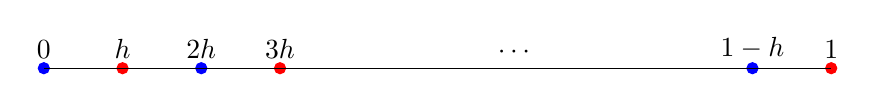
\begin{tikzpicture}
\coordinate (A) at (-5,0);
    \node[above](a) at (A) {$0$};
    \filldraw[blue]  (A) circle (2pt);
\coordinate (B) at (-4,0);
    \node[above](b) at(B) {$h$};
    \filldraw[red] (B) circle (2pt);
\coordinate (C) at (-3,0);
    \node[above](c) at (C) {$2h$};
    \filldraw [blue] (C) circle (2pt);
\coordinate (D) at (-2,0);
    \node[above](d) at (D) {$3h$};
    \filldraw [red] (D) circle (2pt);
\coordinate(E) at (4,0);
    \node[above](e) at (E) {$1-h$};
    \filldraw [blue] (E) circle (2pt);
\coordinate (F) at (5,0);
    \node[above](f) at (F) {$1$};
    \filldraw [red] (F) circle (2pt);
\draw[thin, black](A)--(F);
\node[above](dots) at (1,0) {$\cdots$};
\end{tikzpicture}
\end{center}

The next step is to permute the rows and columns of $A$ according to this coloring, we can represent the permutation easily in the form of a block matrix. 
\beq
P^{-1}AP = \begin{bmatrix} 2I & Q^T\\
Q & 2I
\end{bmatrix}
\eeq
Here $Q$ is some matrix that contains only $0$'s and $-1$'s it represents the connections between blue and red nodes. On the main diagonal there is only $2I$ because no blue node is adjacent to a blue node and no red node is adjacent to a red node. Now we can use the Schur complement for block matrices, to discover something about the characteristic polynomial of $A$.
\beq
\text{det}(\lambda I-A) = \text{det}(P^{-1}(\lambda I-A)P) = \text{det}(\lambda I-P^{-1}AP) = \text{det}((\lambda-2)^2I - Q^TQ)
\eeq

So $\text{det}(A-\lambda I) = q((2-\lambda)^2)$ for some polynomial $q$. This means that if $\lambda$ is eigenvalue for $A$, then $2-\lambda$ is also an eigenvalue of $A$. From this and \eqref{eq:lambdamin} we see that 
\beq
\label{eq:lambdamax}
2 - \sqrt{\frac{2}{N}} \leq \lambda_{\max} \leq 2. 
\eeq

Therefore 
\beq
\kappa \geq \frac{2 - \sqrt{\frac{2}{N}}}{\sqrt{\frac{2}{N}}} = \sqrt{2 N} -1 >\sqrt{N} .
\eeq

We can return to Theorem \ref{thm:conv}, notice that $\frac{\sqrt{x}-1}{\sqrt{x}+1}$ is a decreasing function. We get that 
\beq
\|\bx_* - \bx_k \|_A \leq 2 \left(\frac{\sqrt[4]{N}-1}{\sqrt[4]{N}+1} \right)^k \|\bx_*\|_A.
\eeq

We have the fourth root of $N$, in the coefficient, so this tells us that CG will perform well for our matrices at least until $\sqrt[4]{N}$ starts to get large.

It is possible to make one more improvement on CG, the so called PCG method. This method is very interesting, unfortunately it is \textit{too} interesting for me to cover it in detail. Briefly the idea is to find a different SPD matrix $B = R^TR$ and then look at modified problem 
\begin{align}
\label{eq:precon}
R^{-T}AR^{-1}\by &= R^{-T}\bb\\ \nonumber
\by &= R\bx
\end{align}
This matrix $B$ is called the preconditioner and we will want to select $B$ so that 
\beq
\kappa(R^{-T} A R^{-1}) \ll \kappa(A).
\eeq
When we apply CG to the modified system we will be able to speed up the convergence. The problem of finding a good preconditioner quickly is well known and well known to be difficult. The Incomplete Cholesky factorization is a popular preconditioner, but in general how to select $B$ is an open field of research. 

\printbibliography

\end{document}
